\documentclass{ximera}


\author{Anna Davis} \title{MTH 160 Test 4} 

\begin{document}

\begin{abstract}

\end{abstract}
\maketitle
 \textit{You have 50 minutes to complete this test.  Each answer is worth 1 point.}
 \begin{problem}\label{prob:160test4prob1}
 Find the EXACT values of the six trigonometric functions for angle $\theta$. 
 
 \begin{image}
   
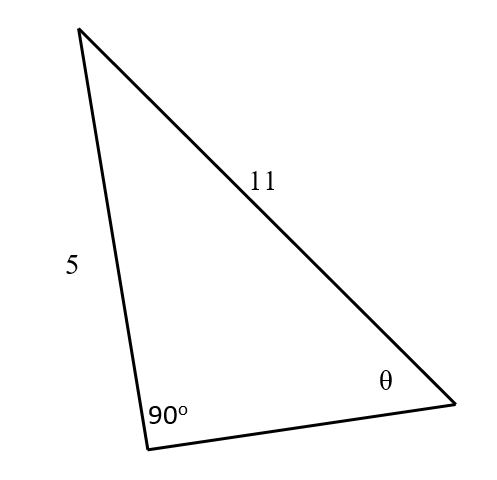
\includegraphics[height=1in]{test4diagram1.jpg}

\end{image}

$$\sin\theta=\answer{5/11},\quad \cos\theta=\answer{\frac{\sqrt{96}}{11}},\quad\tan\theta=\answer{\frac{5}{\sqrt{96}}}$$
$$\csc\theta=\answer{\frac{11}{5}},\quad\sec\theta=\answer{\frac{11}{\sqrt{96}}},\quad\cot\theta=\answer{\frac{\sqrt{96}}{5}}$$

\end{problem}

\begin{problem}\label{prob:160test4prob2}
 Find $x$.  
 
 \begin{image}
   
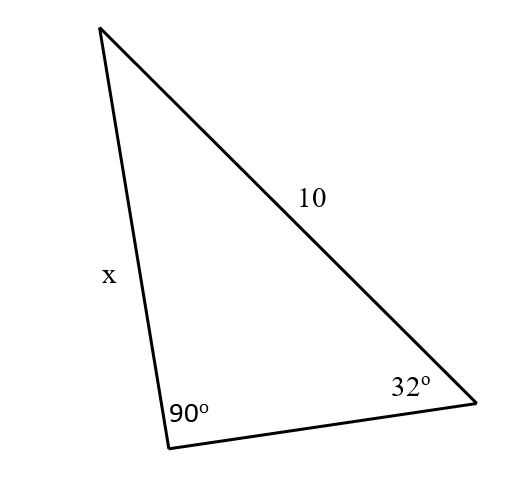
\includegraphics[height=1in]{test4diagram2.jpg}

\end{image}
$$x=\answer[tolerance=0.01]{5.3}$$

\end{problem}

\begin{problem}\label{prob:160test4prob3}
 Find $x$. 
 
 \begin{image}
   
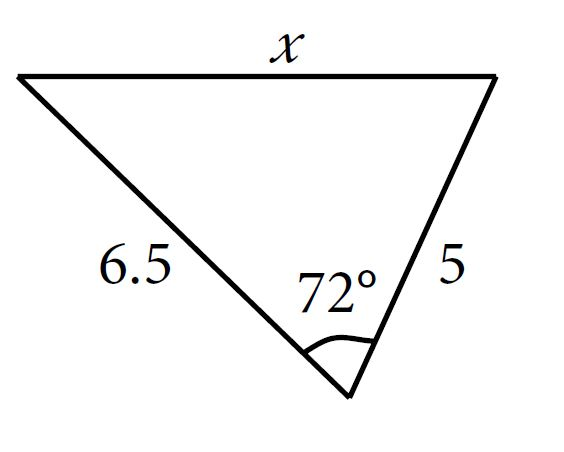
\includegraphics[height=1in]{test4diagram3.jpg}

\end{image}
$$x=\answer[tolerance=0.01]{6.87}$$
\end{problem}

\begin{problem}\label{prob:160test4prob4}
 Find $x$.
 
 \begin{image}
   
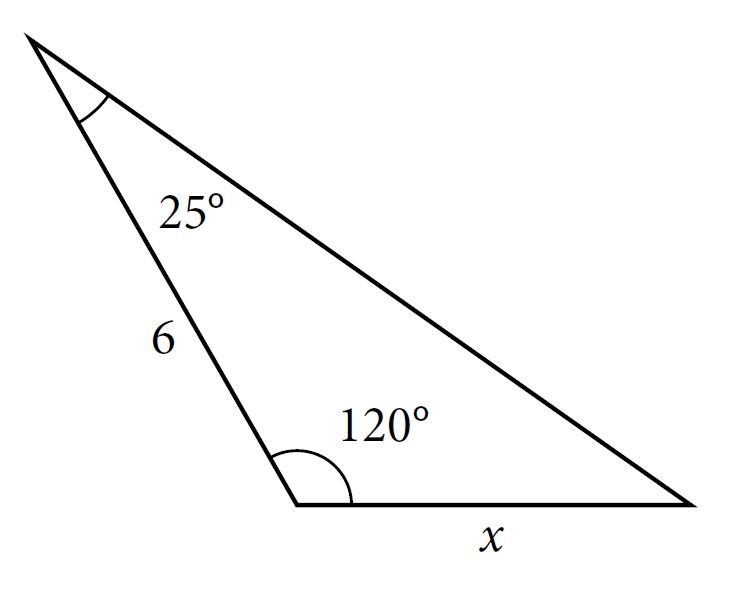
\includegraphics[height=1in]{test4diagram4.jpg}

\end{image}
$$x=\answer[tolerance=0.01]{4.42}$$
\end{problem}

\begin{problem}\label{prob:160test4prob5}
 Find the degree measure of angle $\alpha$.  
 
 \begin{image}
   
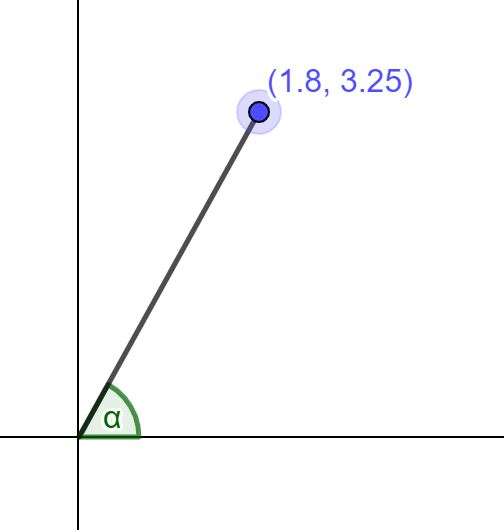
\includegraphics[height=1in]{test4diagram5.jpg}

\end{image}
$$\alpha=\answer[tolerance=0.01]{61}^o$$
\end{problem}

\begin{problem}\label{prob:160test4prob6}
 Find the degree measure of angle $\alpha$.  
 
 \begin{image}
   
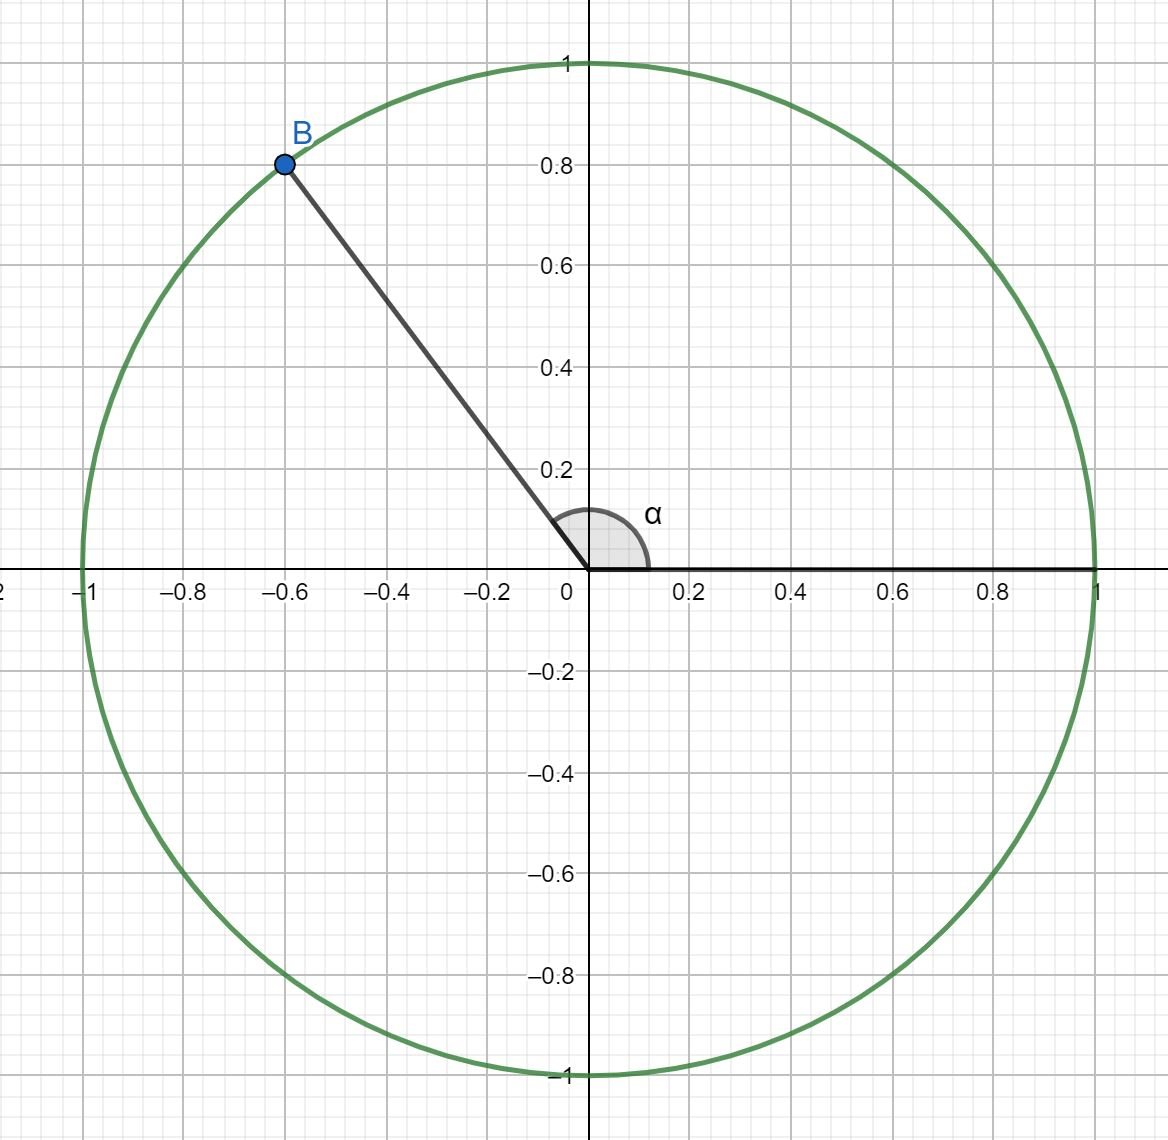
\includegraphics[height=1in]{test4diagram8.jpg}

\end{image}
$$\alpha=\answer[tolerance=0.01]{126.87}^o$$

\end{problem}

\begin{problem}\label{prob:160test4prob7}
 Find $y$.
 
 \begin{image}
   
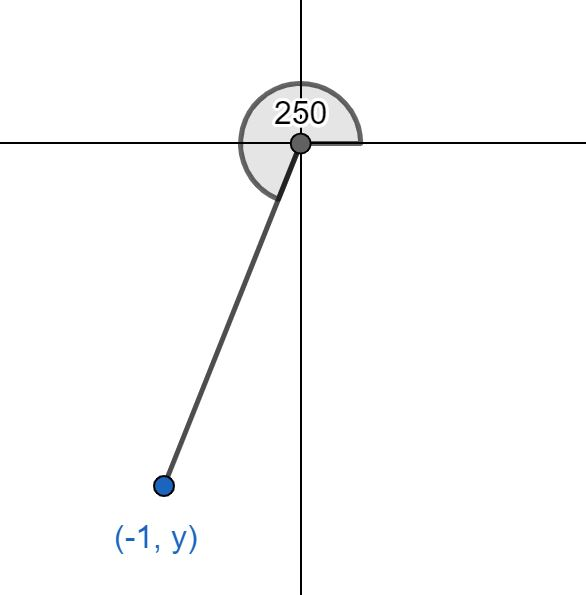
\includegraphics[height=1in]{test4diagram9.jpg}

\end{image}
$$y=\answer[tolerance=0.01]{-2.75}$$

\end{problem}
 
 \end{document}